\section{Создание мобильного приложения}

В рамках данной аттестационной работы было разработано кроссплатформенное мобильное приложение системы вероятностного моделирования с использованием фреймворка Apache Cordova. Данное приложение можно скомпилировать на множество платформ, поддерживаемых Apache Cordova, в частности это: Tizen, webOS, Android, iOS, Blackberry, Samsung Bada и Windows Phone. Тестировалось приложение на платформе Android 4.0.4 Ice Cream Sandwich.

\subsection{Настройка окружения}
Перед началом процесса разработки мобильного приложения необходимо настроить окружение, установить необходимые библиотеки и средства разработки. Для начала, необходимо убедиться, что NodeJS уже установлен и доступен для использования:
\begin{lstlisting}
 $ nodejs --version
 $ npm --version
\end{lstlisting}

Обе команды необходимо выполнить в командной строке и убедиться в том, что они успешно выполнились. В противном случае необходимо установить необходимые программы. Далее, установим необходимые библиотеки и их зависимости:
\begin{lstlisting}
 $ npm install -g cordova
\end{lstlisting}

Данная команда скачает из репозитория npm файл package.json для проекта cordova, создаст файлы, относящиеся к проекту, установит все зависимости, необходимые для корректной работы данного фреймворка, а также создаст ссылки на исполняемые файлы. Результат работы этой команды отображен на рисунке \ref{npm_cordova}. После завершения скрипта в нашей системе появится возможность использовать Cordova CLI из любого места за счет глобальной пролинковки (атрибут -g в команде установки).

\begin{figure}[ht]
\center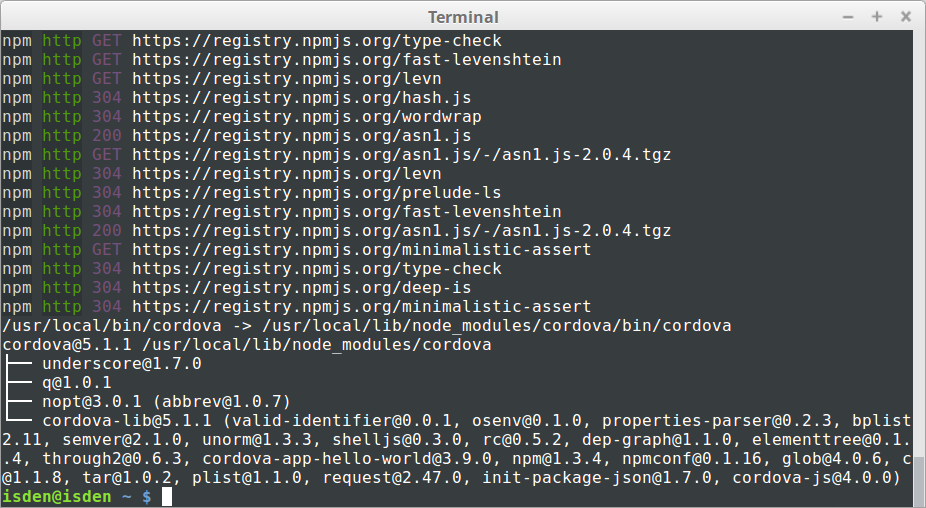
\includegraphics[width=0.9\textwidth]{npm_cordova}
\caption{Результат установки cordova}\label{npm_cordova}
\end{figure}

Для сборки проекта под Android необходимо установить и настроить Java SDK и Android SDK. Для этого скачиваем последние версии наборов разработки с официального сайта Oracle\cite{cordova:java_sdk} и официального сайта Google\cite{cordova:android_sdk}. Установка Java SDK не отличается ничем примечательным. После установки необходимо убедиться что правильно задана переменная окружения JAVA\_HOME.

Установка Android SDK отличается на различных платформах. Например, под ОС Windows необходимо запустить инсталлятор и следовать полученным инструкциям от мастера установки. Под ОС GNU\\Linux дистрибутив распространяется в качестве простого архива, который достаточно просто распаковать. После установки запускаем утилиту настройки \textit{android}, которая находится в каталоге tools. Для сборки проекта в Apache Cordova необходимы Build Tools последних версии, а также Platform Tools и Tools. Также необходимо установить SDK Platform версии не ниже 22. Пометим флажками для установки нужные компоненты (рисунок \ref{android_sdk}), прочтем лицензионное соглашение и ожидаем окончания процесса скачивания и установки. После проведения данных манипуляций, необходимо убедиться в том, задана переменная ANDROID\_HOME, которая указывает расположение Android SDK. что в переменной PATH добавлен путь к каталогам tools и platform-tools. Теперь все готово для начала процесса разработки.
\begin{figure}[ht]
\center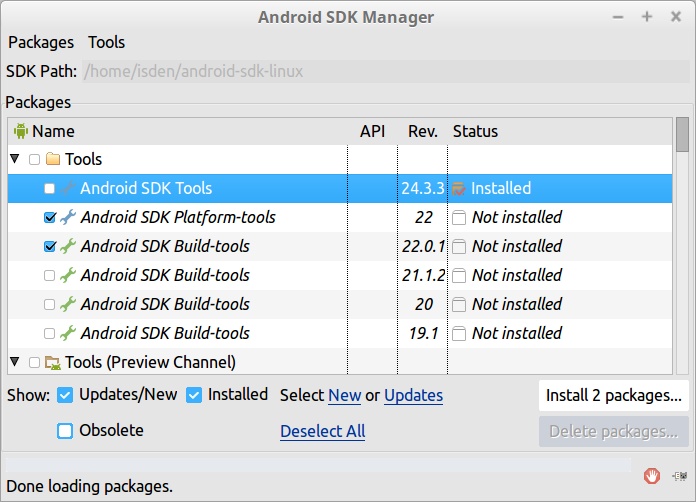
\includegraphics[width=0.9\textwidth]{android_sdk}
\caption{Окно настройки средств разработки Android}\label{android_sdk}
\end{figure}

\subsection{Адаптация приложения}
Для начала работ по переносу веб-приложения на мобильные устройства необходимо создать базовую структуру каталогов. Для этого воспользуемся командой:
\begin{lstlisting}
 $ cordova create adhoc-system
 $ cordova platform add android
\end{lstlisting}

Первая команда создаст необходимые для работы каталоги и файлы конфигурации. Структура каталогов отображена на рисунке \ref{cordova_structure}. Директория \textit{platforms} включает в себя раздельный код под каждую из используемых платформ. Компилируется каждый раз при выполнении сборки. В директории \textit{plugins} находятся подключаемые библиотеки Cordova, используемые в приложении. Например для работы с консолью вывода устройства. Каталог www представляет собой наше веб-приложение. Также в корне проекта есть файл \textit{config.xml}, отвечающий за основные настройки приложения. Этот файл является самой важной частью проекта на основе Apache Cordova. Он включает в себя ссылки на ресурсы приложения, устанавливает необходимые разрешения и настраивает параметры для каждой из платформ (например поведение статусной строки). Идентификатор приложения (bundle) и информация об издателе должна быть также указана в файле \textit{config.xml}.
\begin{figure}[ht]
\center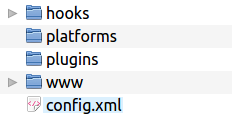
\includegraphics[width=0.9\textwidth]{cordova_structure}
\caption{Структура проекта Apache Cordova}\label{cordova_structure}
\end{figure}

Плагины в Apache Cordova представляют собой пакеты, которые позволяют внедрить нативный код в приложение и управлять методами из Cordova Web View. Все основные функции Cordova API реализованы при помощи плагинов, которые предоставляют доступ к возможностям и функциям устройства и платформы, которые недоступны обычному веб-приложению: например доступ к камере, NFC, уведомления в в статусной строке и даже доступ к отпечаткам пальцев, при наличии данной возможности в аппарате. В данной работе плагин не был реализован, хватило встроенных возможностей Cordova API.

Существует отдельный репозиторий Cordova плагинов. Все плагины обычно имеют документацию и примеры использования, а также содержат исходный код на GitHub. Для отладки был подключен плагин cordova-plugin-console, который позволяет дублировать вывод команды console.log в лог отладки приложения, доступный средствами отладки конкретной платформы. Его установка производится следующей инструкцией:
\begin{lstlisting}
 cordova plugin add cordova-plugin-console
\end{lstlisting}

После всех приготовлений можно переносить код написанного с использованием AngularJS приложения в каталог www. Так как сборка будет производиться без использования bower, то вручную предварительно выполним команду \textit{bower install}. 

Для мобильных телефонов, имеющих низкое разрешение экрана, с целью компактно разместить компоненты на экране, были написаны новые таблицы стилей. Для этого был продуман и создан отдельный дизайн веб-страниц. Этот дизайн обеспечивает корректное отображение представлений приложения на различных устройствах, запускающих мобильное приложение и динамически подстраивающийся под заданные размеры экрана аппарата. Таким образом, приложение удобно просматривается с устройств различных разрешений и форматов. Теперь не нужно реализовывать отдельные версии представлений для отдельных видов устройств. Одно представление может работать как на устаревших аппаратах, так и на современных экранах, обладающих высокой плотностью пикселей. Такой подход практикуют большинство современных разработчиков мобильных приложений и веб-мастеров. Пример стиля для адаптивного дизайна отображен ниже:
\begin{lstlisting}
  #sidebar {
    position: absolute;
    right: 0;
  }

  @media screen and (max-width: 700px) {
    #sidebar {
      position: fixed;
      bottom: 0;
      right: auto;
      width: 100%;
    }
    #sidebar a {
      float: left;
    }
    body {
      padding-bottom: 100px;
    }
  }
\end{lstlisting}

После создания проекта и проведенной адаптации приложения к мобильному виду, все готово для сборки приложения под различные платформы.

\subsection{Сборка приложения}
Сборку приложения будем производить на примере Android. 